%%%%%%%%%%%%%%%%%%%%%%%%%%%%%%%%%%%%%%%%%%%%%%%%%%%%%%%%%%%%%%
%% Carlos Segarra's Beamer Presentation Template. All credits
%% to Vincent Labatut from whom I took the template and added
%% my own flavour to it. Kudos to <vincent.labatut@univ-avignon.fr>
%%%%%%%%%%%%%%%%%%%%%%%%%%%%%%%%%%%%%%%%%%%%%%%%%%%%%%%%%%%%%%
% setup Beamer
\documentclass[10pt,    % default is 11pt, use 10pt for more compact slides
%    handout,            % collapse all overlays (=animations) and video-invert console text
    english,            % presentation language (theme supports only french & english)
    xcolor=table,       % colors in the tables
    envcountsect,        % include section number in theorem numbers
    aspectratio=169     % Using 16:9 aspect ratio because 2019
]{beamer}

%%%%%%%%%%%%%%%%%%%%%%%%%%%%%%%%%%%%%%%%%%%%%%%%%%%%%%%%%%%%%%
% setup the theme
%\usepackage{au/sty/beamerthemeAU}         % no option at all
\usepackage[light]{csg-temp/sty/beamerthemeAU}   % the "light" option only changes the title and section pages

%%%%%%%%%%%%%%%%%%%%%%%%%%%%%%%%%%%%%%%%%%%%%%%%%%%%%%%%%%%%%%
% setup side notes
\usepackage{pgfpages}                                   % comment all 3 below lines to hide notes
%\setbeameroption{show notes}                           % alternate content and note slides
%\setbeameroption{show only notes}                      % only note slides
%\setbeameroption{show notes on second screen=right}    % dualscreen: right, left, top, bottom
%\usepackage{enumitem}

%%%%%%%%%%%%%%%%%%%%%%%%%%%%%%%%%%%%%%%%%%%%%%%%%%%%%%%%%%%%%%
% name of the biblatex file
\addbibresource{biblio.bib}

%%%%%%%%%%%%%%%%%%%%%%%%%%%%%%%%%%%%%%%%%%%%%%%%%%%%%%%%%%%%%%
% External Packages
\usepackage{datenumber}
\usepackage{varwidth}

% Math Mode
%\usepackage{algorithm}
%\usepackage{algorithmic}
%\usepackage{algorithm2e}
%\usepackage{multicol}
%\usepackage[noend]{algpseudocode}

%%%%%%%%%%%%%%%%%%%%%%%%%%%%%%%%%%%%%%%%%%%%%%%%%%%%%%%%%%%%%%
% title and subtitle of the presentation (the latter is optional)
\subtitle{Discrete and Algorithmic Geometry} % leave empty if no subtitle
\title[The Bin Packing Problem] % leave empty for no title in footer
    {\normalsize Discrete and Algorithmic Geometry \\ \Large The Bin Packing Problem: \\ \Large Definition and Applications}
\subtitle{Master in Advanced Mathematics and Mathematical Engineering - MAMME}
%%%%%%%%%%%%%%%%%%%%%%%%%%%%%%%%%%%%%%%%%%%%%%%%%%%%%%%%%%%%%%
% date of the presentation (leave empty for no date, default is today)
\date[\today] % leave empty for no date in footer
    {\datedayname, \today}
%%%%%%%%%%%%%%%%%%%%%%%%%%%%%%%%%%%%%%%%%%%%%%%%%%%%%%%%%%%%%%
% authors and their affiliations (the latter is optional)
\author[] % leave empty for no author in footer
{Carlos Segarra - \texttt{carlos.segarra@estudiant.upc.edu}}
%{\inst{1} Computer Science Lab, Avignon University -- LIA EA 4128 \texttt{\{firstname.lastname\}@univ-avignon.fr}
%\and \inst{2} Institute of Disruptive Innovation, University of Excellence \texttt{\{firstname.lastname\}@univ-excell.fr}
%}
%%%%%%%%%%%%%%%%%%%%%%%%%%%%%%%%%%%%%%%%%%%%%%%%%%%%%%%%%%%%%%
% optional: additional logo (ex. lab)
%\titlegraphic{\includegraphics[width=3cm,]{images/logo_FME.png}}
% if you want several logos, put them in a box
%\titlegraphic{\parbox{3cm}{\includegraphics[width=3cm,]{images/ceri_logo.pdf}\newline\includegraphics[width=3cm,]{images/lia_logo.pdf}}}
%%%%%%%%%%%%%%%%%%%%%%%%%%%%%%%%%%%%%%%%%%%%%%%%%%%%%%%%%%%%%%

%%%%%%%%%%%%%%%%%%%%%%%%%%%%%%%%%%%%%%%%%%%%%%%%%%%%%%%%%%%%%
% Presentation speciphic packages
% \usepackage{multicol}
% \usepackage[titles]{tocloft}
% \renewcommand{\cftchapfont}{\normalfont\bfseries}
\usetikzlibrary{decorations.pathmorphing, patterns}
\usepackage{tabularx}
\newcolumntype{L}[1]{>{\raggedright\arraybackslash}p{#1}}
\newcolumntype{C}[1]{>{\centering\arraybackslash}p{#1}}
\newcolumntype{R}[1]{>{\raggedleft\arraybackslash}p{#1}}
%%%%%%%%%%%%%%%%%%%%%%%%%%%%%%%%%%%%%%%%%%%%%%%%%%%%%%%%%%%%%

%%%%%%%%%%%%%%%%%%%%%%%%%%%%%%%%%%%%%%%%%%%%%%%%%%%%%%%%%%%%%%
\begin{document}
%%% title page
\begin{frame}
  \titlepage
\end{frame}

\begin{frame}
    \frametitle{Bin Packing Problem}
    \framesubtitle{Definition, History, and Examples}

    \begin{block}{Problem Statement}
        Suppose we have $n$ objects, each of a given size, and some bins of equal capacity. We want to assign the objects tot he bins using as few bins as possible. Of course the total size of the objects assigned to one bin should not exceed its capacity.$[1]$
    \end{block}


    \small
    \begin{description}
        \item $[1]$ Korte, Bernhard; Vygen, Jens (2006). \textbf{\textit{"Bin-Packing"}}. Combinatorial Optimization: Theory and Algorithms. Algorithms and Combinatorics 21. Springer. pp. 426–441.
    \end{description}

\end{frame}

\begin{frame}
    \frametitle{Bin Packing Problem}
    \framesubtitle{Definition, History, and Examples}

    \begin{alertblock}{Complexity and Applications}
        The Bin Packing decision problem is \textbf{NP-complete}. The formulation is applicable to a variety of real-world problems and admits several reformulations.
    \end{alertblock}

    \begin{enumerate}
        \item Online bin packing.
        \item Filling up trucks in a logistics environment.
        \item Creating file backups in media.
        \item Knapsack problem (one bin and each item has cost and value).
        \item Virtual Machine placement in a data center.
    \end{enumerate}

\end{frame}

\begin{frame}
    \frametitle{Bin Packing Problem}
    \framesubtitle{Formal Statement}

    \vspace{-10pt}

    Given a set of bins $S_1, S_2, \dots$ with the same size $V$ and a list of $n$ items with sizes $a_1, \dots, a_n$ to pack,
    \begin{equation*}
        \begin{aligned}
            \text{minimize } & B = \sum\limits_{i = 1}^{n} y_i \\
            \text{subject to } & B \geq 1 \\
            & \sum\limits_{j = 1}^{n}a_jx_{ij} \leq V y_i, \quad \quad \forall i \in \lbrace 1, \dots, n\rbrace \\
            & \sum_{i = 1}^n x_{ij} = 1 \qquad \qquad x_{ij}, y_i \in \lbrace 0, 1 \rbrace \\
            %& x_i \in \lbrace 0, 1 \rbrace
        \end{aligned}
    \end{equation*}
    \hspace{20pt} where $y_i = 1$ if bin $S_i$ is used and $x_{ij} = 1$ if item $a_j$ is put into bin $S_i$.

\end{frame}

\begin{frame}
    \frametitle{Bin Packing in Geometry}
    \framesubtitle{2D Bin Packing}
    
    \begin{itemize}
        \item The classic representation of the Bin Packing problem has a straight-forward 2D geometric representation.
    \end{itemize}

    \vspace{-10pt}

    \begin{figure}
        \centering
        \resizebox{0.8\linewidth}{!}{
        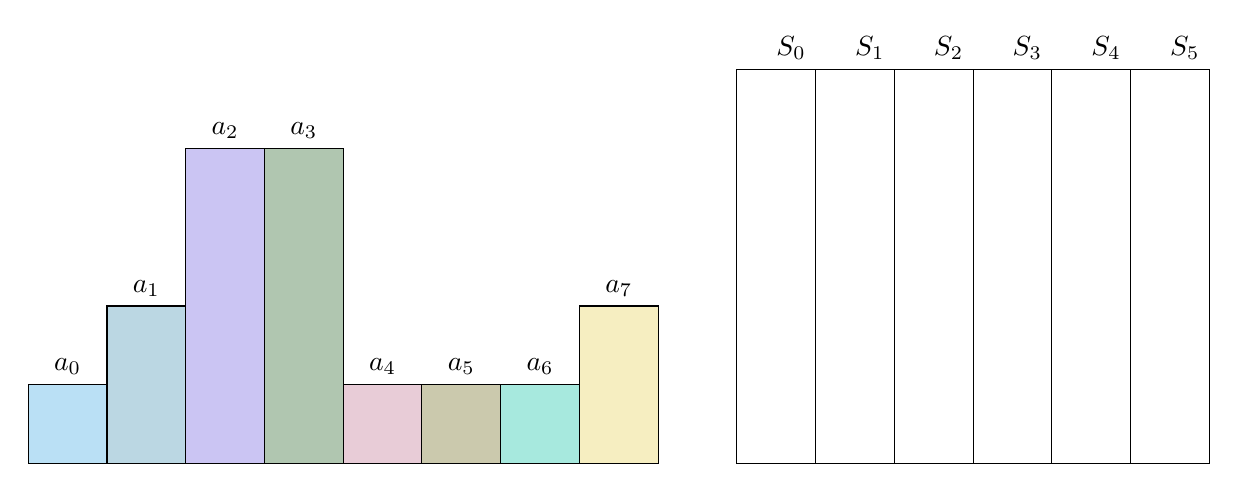
\begin{tikzpicture}
            \foreach \x in {0,...,7}
            {
                \begin{scope}
                    \pgfmathparse{250*rnd+5}
                    \edef\tmpi{\pgfmathresult}
                    \pgfmathparse{210*rnd+45}
                    \edef\tmpii{\pgfmathresult}
                    \pgfmathparse{230*rnd+25}
                    \edef\tmpiii{\pgfmathresult}
                    \pgfmathparse{0.75*rnd+0.25}
                    \edef\opac{\pgfmathresult}
                    \definecolor{MyColor}{RGB}{\tmpi,\tmpii,\tmpiii}    
                    \pgfmathparse{int(4*rnd) + 1}
                    \edef\rndheight{\pgfmathresult}
                    %\draw[fill=MyColor!40] (0,\x*0.5) rectangle (1,0.5*\x + .5) node[pos=.5] (orig-\x) {$a_{\x}$};
                    \draw[fill=MyColor!40] (\x, 0) rectangle (\x + 1, \rndheight) node[anchor=south] (orig-\x) at (\x + 0.5, \rndheight) {$a_{\x}$}; 
                \end{scope}
            }
            \foreach \y in {0,...,5}
            {
                \begin{scope}
                    \draw (9 + \y, 0) rectangle (10 + \y, 5) node[anchor=south east] (bin-\y) {$S_{\y}$};
                    %\draw (5 + \y, 0) rectangle (6 + \y, \tmpi);
                \end{scope}
            }
        \end{tikzpicture}
        }
        %\caption{Classsic representation of the bin packing problem.}
    \end{figure}
\end{frame}


\begin{frame}
    \frametitle{Solving BP: Greedy Approximation Algorithms}
    \framesubtitle{First Fit (FF), First Fit Decreasing (FFD)}

    \begin{columns}
        \begin{column}{.45\textwidth}
            \textbf{First Fit Algorithm:}
            \begin{itemize}
                \item Try to fit each element in the current set of opened bins. If it fits in none, open a new bin.
                \item Runtime $\mathcal{O}(n \log n)$
                \item Approximation factor: $1.7$
            \end{itemize}
            \textbf{First Fit Decreasing Algorithm:}
            \begin{itemize}
                \item Order the elements to sort, and apply First Fit.
                \item Runtime $\mathcal{O}(n \log n)$
                \item Approximation factor: $1.222$
            \end{itemize}
        \end{column}
        \begin{column}{.45\textwidth}
            \begin{algorithm2e}[H]
                \KwIn{Some Input}
                \While{$item \gets S.\text{pop}()$}
                {
                    \For{$bin \in B$}
                    {
                        \If{$\text{fits}(item, bin)$}
                        {
                            $\text{put}(item, bin)$\;
                            \textbf{break}\;
                        }
                    }
                    \Else
                    {
                        $\text{put}(item, \text{new}(bin))$\;
                    }
                    % If it does not fit in any bin, open new one
                }
                \caption{First Fit Algorithm}
            \end{algorithm2e}
        \end{column}
    \end{columns}

    \tiny
    \begin{description}
        \item $[1]$ Maxence Delorme, Manuel Iori, Silvano Martello. \textbf{\textit{"Bin-Packing and Cutting Stock Problems: Mathematical Models and Exact Algorithms"}}.  Section 2.3.
    \end{description}
\end{frame}

\begin{frame}
    \frametitle{Modern Applications: VM Placement}

    \begin{figure}[h!]
        \centering
        \resizebox{0.8\linewidth}{!}{
        \begin{tikzpicture}
            \draw[dashed] (0,0) rectangle (4, 6);
            \draw[dashed] (8,0) rectangle (12, 6);
            \draw (8.15,0.5) rectangle (8.65, 5.5);
            \draw (8.7,0.5) rectangle (8.95, 5.5);
            \draw (9,0.5) rectangle (9.45, 5.5);
            \draw (9.5,0.5) rectangle (10.5, 5.5);
        \end{tikzpicture}
        }
    \end{figure}

\end{frame}


\section*{Questions \& Observations}
\sectionframe

\end{document}
